\section{Contextualization}

Documents are at the core of corporate society, and they often hold immeasurable value, representing contracts, employment relationships, loans, and identities. Recently, as technology becomes more accessible, documents have become increasingly more digital, some never being printed on paper. These documents often have all important information already separated in the file's metadata and require no extra intelligence to classify or extract the information. However, many organizations still receive documents in physical form, for example, when dealing directly with individual customers, which makes full digitization impractical in many cases.

In such a scenario, the company must have a document understanding pipeline, where the document is approved regarding its form (verifying if the client sent the right type of document) and the information is extracted to support business decision-making, as seen in \refFig{fig:compliance}. This pipeline has historically been executed by humans. Between the start of the digital revolution and the popularization of \gls{OCR} engines~\cite{kay_tesseract_2007, doctr2021}, the typist profession was highly prevalent, with workers responsible for manually entering information from physical documents into digital systems. Moreover, the classification and information extraction were done by back office analysts, who spent their workforce reading and verifying if the document met the company's compliance rules. Today, with current technology, especially with the popularization of neural networks, this manual document pipeline has become unthinkable in big companies, as it is inefficient in both time and cost. This work focuses on automatic document classification.

\begin{figure}[htbp]
%\isPreprints{\centering}{} % Only used for preprints
\label{fig:compliance}
\centering
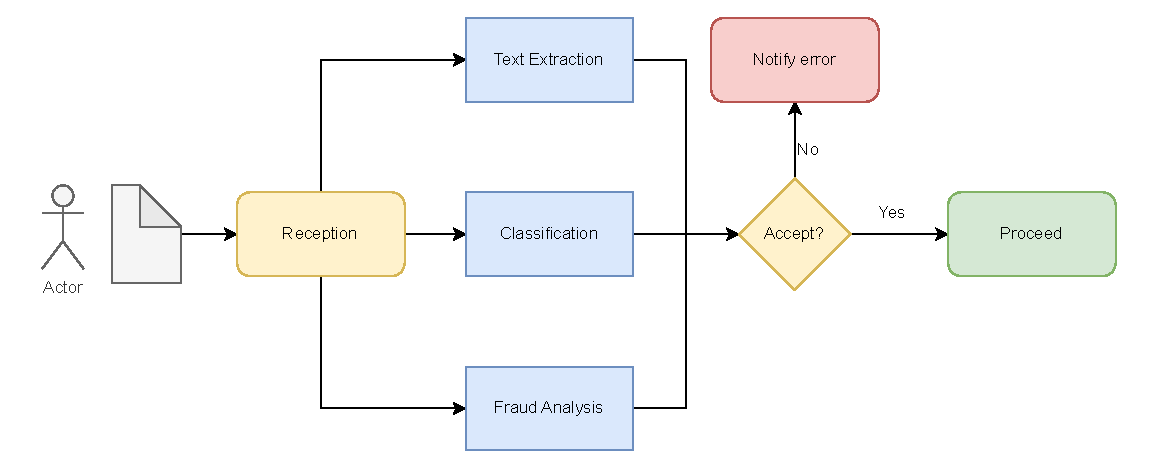
\includegraphics[width=1\linewidth]{images/diagrama-compliance.drawio.pdf}
\caption{Simplified view of a document compliance pipeline. In this diagram, text extraction, document classification and fraud analysis are being used together to decide upon the acceptance of the recieved document.}
\end{figure}

Document Classification is defined by the the categorization of documents into predefined classes~\cite{liu_document_2021}. \gls{DIC} is a more specialized task in which textual information is not directly available, and the input often consists of photos or scans of physical documents. Therefore, if the text of the document is ever required, this text should be extracted with \gls{OCR} algorithms. \gls{AI} and \gls{DL} techniques can automate document classification by leveraging traditional classification networks. The model solution may analyze just the image, which can cut the computational cost of the overall solution by not using an \gls{OCR} algorithm. Sometimes, however, the image may not give enough information to make a proper decision, so models may also be modeled to classify based on text information, or even mix both in a multimodal solution. This problem is already known and well studied. Bakkali et al.~\cite{bakkali_eaml_2021} achieved $97.70\%$ accuracy on the RVL-CDIP dataset~\cite{harley2015rvlcdip}, a popular document classification dataset.

The problem arises when previously accepted documents change in form or when entirely new document classes, not previously considered, must be handled and categorized. In such cases, models are typically retrained, as traditional classification networks may struggle to generalize to new document layouts or entirely new classes. Traditional \gls{DL} classification methods require a predefined set of labels and cannot output a label outside the original training set. Therefore, introducing new labels to the model means retraining the model, changing the output layer into a wider one with more options. Very often, this also means weeks or months of data engineering, labeling, and model training. The alternative is to use \gls{ZSL} techniques, which allow models to generalize to classes that were not seen during training~\cite{xian_zero-shot_2019}.

% \red{DIAGRAMA ZSL VS TRADICIONAL AQUI}

\section{Problem Description}
\label{sec:problem}

This work focuses on the \gls{ZSL} on \gls{DIC}, where the model must correctly classify a document image class that was not in the training set and therefore previously unseen by the model. \gls{ZSL} techniques enable a single model to address multiple classification problems, as they are not limited by the classes used in training. Most \gls{ZSL} systems work by semantically mapping the elements into a feature space, where elements from the same class are all clustered together, and different classes are placed far apart. To build a reliable \gls{ZSL} system, it is necessary to identify a set of features that serve as robust representations, ensuring that documents share features if, and only if, they belong to the same class. With \gls{DL}, this could also demand a dataset with a wide variety of classes, enough so that the model learns what makes two documents similar or different. These conditions allow \gls{ZSL} models to group together documents, even if they were completely unseen during training. Nonetheless, not every classification dataset can be easily used in an effective \gls{ZSL} solution. The lack of a specialized dataset is one of the biggest challenges in document-image \gls{ZSL} classification.

In consequence, another main challenge in image-based document \gls{ZSL} classification is the lack of a state-of-the-art methodology. Due to the challenge in achieving \gls{ZSL} classification with the currently available datasets, most works tackle the problem by their own methodology and are often incomparable to the ones that came before~\cite{sinha2024cica}, unlike traditional classification and information extraction that have a widely accepted framework and baseline approaches. Many works also use pretrained \gls{LLM}~\cite{scius2024zeroshot}, leveraging their previous knowledge as a tool to achieve zero-shot learning with a fine-tuning framework, which limits the cost-efficiency achievable with this strategy.

But there are a few known obstacles in zero-shot document classification. First, existing datasets do not enforce disjoint class splits between training and testing, nor do they provide enough information to train an efficient \gls{ZSL} model from scratch. Second, there is an absence of a well-established, state-of-the-art classification framework capable of operating under zero-shot constraints.

\section{About this work}

Following this line, this work proposes a new framework for tackling \gls{ZSL} document classification: \gls{VDM}. By leveraging metric learning techniques, documents with similar patterns can be identified and grouped into the same class/group, even if their class was not seen before during training. Through this method, \gls{VDM} shows itself as a zero-shot alternative for the identification of documents that are visually equivalent, as a matching problem. In other words, \gls{VDM} can be handled as a binary classification problem.

This work makes several key contributions, i.e.:
\begin{enumerate}
    \item Introduces a novel visual-only document image dataset specifically designed for the task of document ZSL classification, enabling the development and evaluation of models in this domain.
    \item Proposes a \gls{VDM} approach, based on image similarity, leveraging zero-shot learning techniques to generalize across unseen document layouts. This strategy enables generalization to previously unseen classes without additional intervention on the model itself.
    \item Delivers a systematic evaluation of well established backbones in the context of zero-shot document layout matching, offering valuable benchmarks for future research.
\end{enumerate}

This paper is structured as follows: \refCap{2-Teorica} lays out the theoretical foundation of this work. \refCap{3-TrabalhosRelacionados} reviews the state of the art in zero-shot learning and visually-rich document understanding, highlighting existing methods and their limitations. \refCap{4-Metodologia} presents the proposed \gls{LA-ZSL} for \gls{VDM}, detailing its architecture, components, and underlying learning paradigm. \refCap{5-Resultados} describes the experimental setup, including datasets, evaluation metrics, and baseline comparisons, followed by a comprehensive analysis of the results. Finally, \refCap{6-Conclusao} concludes the article by summarizing the contributions, discussing potential applications, and outlining future research directions, and the timeline of this Master's research.

